\chapter{Description of the GUI}
\paragraph{This chapter describes how to use the graphical user interface of the NoBeard virtual machine and serves at the same time as a user manual. The application is developed as simple as possible to use. With the three main tools the user can load and run NoBeard object files, debugging running programs and get a whole view of the data memory.}
\begin{center}
	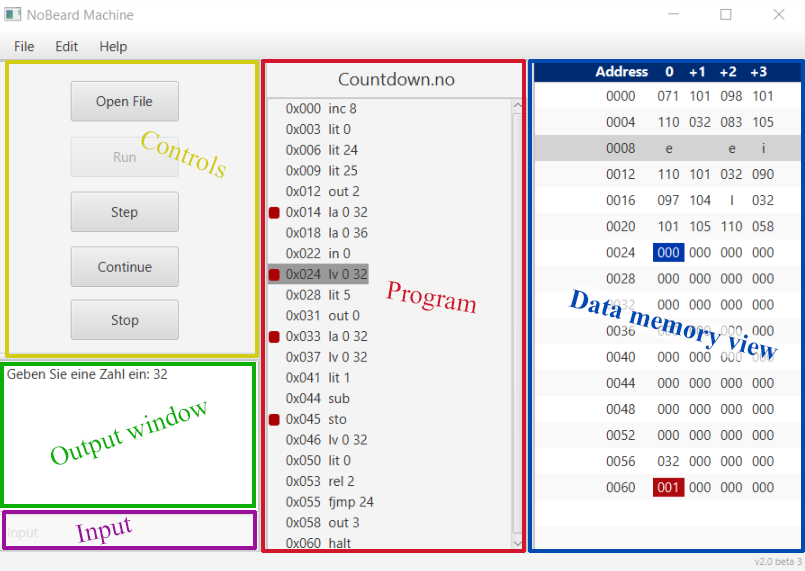
\includegraphics[scale=.90]{images/screenshot-0.png}
\end{center}
\section{Loading \& Running a program}
\paragraph{By starting the user interface, a NoBeard object file has to be loaded by a click on the “open file” button. Than the user can choose the desired file. Afterward, the window shows the content and the title of the opened program which is now executable.}

\paragraph{The content lists instructions with the belonging addresses and operators. By hitting the “Run” button, the machine executes the loaded program. Under the control buttons there is a window which simulates a terminal where the user can see the outputs of the running program. If the program runs against an input instruction, the machine stops and requests the user for an input which can be done under the output window. To submit an input, the Enter key has to be pressed.}

\begin{figure}[h] 
	\centering
	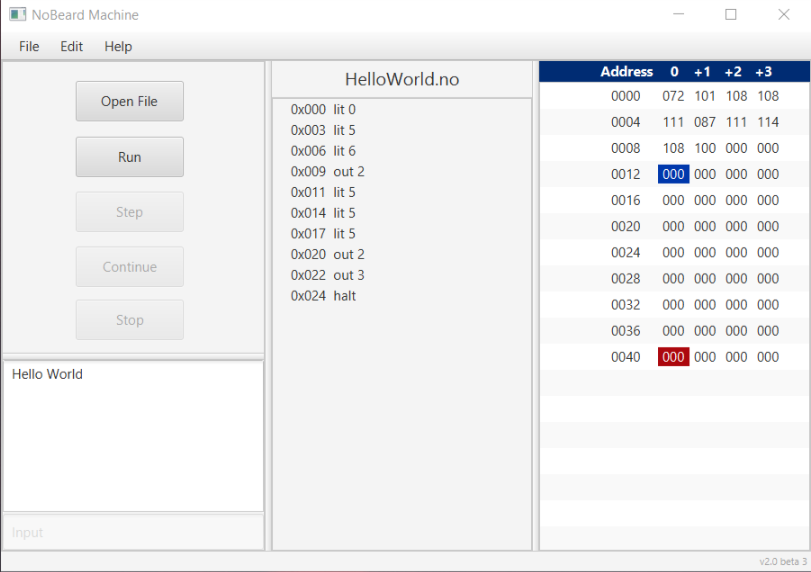
\includegraphics[scale=.75]{images/screenshot-1.png}
	\caption{Executed "Hello World" program}
\end{figure}

\section{Debugging}
\paragraph{To debug a program the user has to set breakpoints. These breakpoints can be placed by clicking on the studied address. If a breakpoint has been placed and the program is about to start, it runs only until the line where the breakpoint has been set.}

\paragraph{Than the user is able to step one line further or jump to the next breakpoint. Stepping is handled by the “Step” button as shown in the following picture. By clicking on the “Continue” button, the program runs from the current line until the next breakpoint. If there is not any breakpoint left from the current line, it runs until the end of file. Optionally, the user is able to stop the program during the execution. This could be achieved by the “Stop” button.}

\begin{figure}[h] 
	\centering
	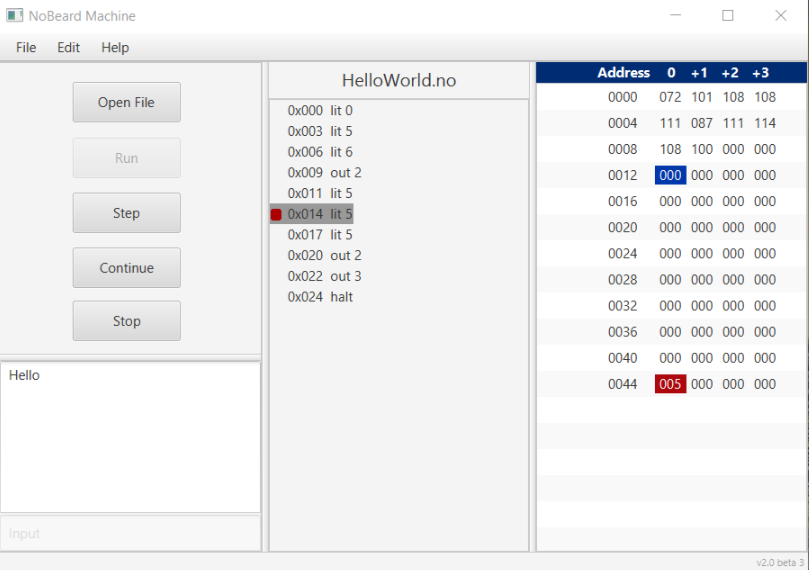
\includegraphics[scale=.75]{images/screenshot-2.png}
	\caption{Debugging the "Hello World" program}
\end{figure}

\section{Data Visualization}
\paragraph{On the right side of the window is the visualisation of the data memory view in a list form. This view lists data byte wise from the data memory of the machine. Each line of the list view has a content of an address given in decimal notation following by four bytes raw data. The memory is separated in two parts. The list starts on the top with the string constants followed by stack frames of the currently running functions. While the frame pointer is highlighted with a blue background, the stack pointer is signed with a red background. The user has also the possibility to convert confused raw data to characters or integers.}
\begin{figure}[h] 
	\centering
	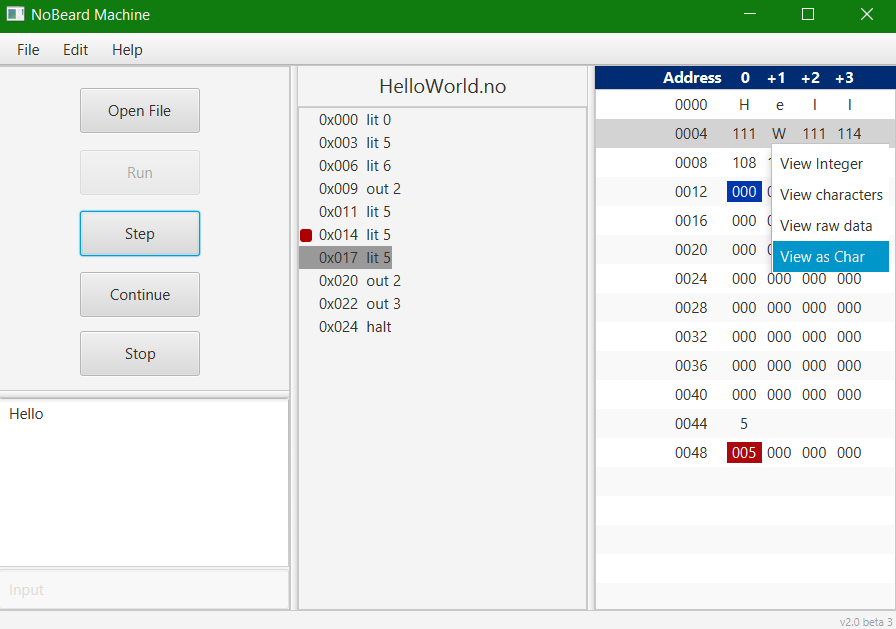
\includegraphics[scale=.60]{images/screenshot-3.png}
	\caption{Converting data to characters}
\end{figure}
\paragraph{With a right click on the selected line of the list, a context menu could be opened. This menu includes following functions: showing integer, characters of the whole line, a single character or converting back the line to raw data. To make the conversion from raw data to alphanumeric characters or integers more easy and fast, a multi selection function is developed for the list of the data memory.}